\hyphenation{se-para-tion}
\hyphenation{theo-re-ti-cal}
\hyphenation{handed-ness}
\hyphenation{fo-llo-wing}
\hyphenation{ac-cor-ding}

%______________________ Theory ______________________
\chapter{The LHC Accelerator and the CMS Experiment}\label{ch:lhcandcms}
In the 1960s Peter Higgs and others {\color{red}\ital{need ref}} put up the finishing touches on a theory combining three of the four fundamental forces. This theory became to be known as the Standard Model (SM) of particles physics. It predicted the existence of several particles which were discovered in the following decades. However, one particle was proving to be elusive, the so-called Higgs bosson. With this in mind the European Organization for Nuclear Research (CERN) started plans to build an accelerator large enough to be able to find this elusive particle. Hence, the Large Hadron Collider (LHC) was born. 

\section{The LHC Accelerator}
The LHC, the biggest particle accelerator {\rojo{built}} by mankind to date, was built in the french-Swiss border outside of Geneva, Switzerland. A circular ring of 27 km built at the European Council for Nuclear Research (CERN) using the same tunnel as the large electron-positron collider. It accelerates two beams of protons in opposite directions until they reach an energy of 7 Tera electron Volts (TeV), making the center of mass energy 14 TeV. 
 

\begin{figure}[!h]
	\centering
	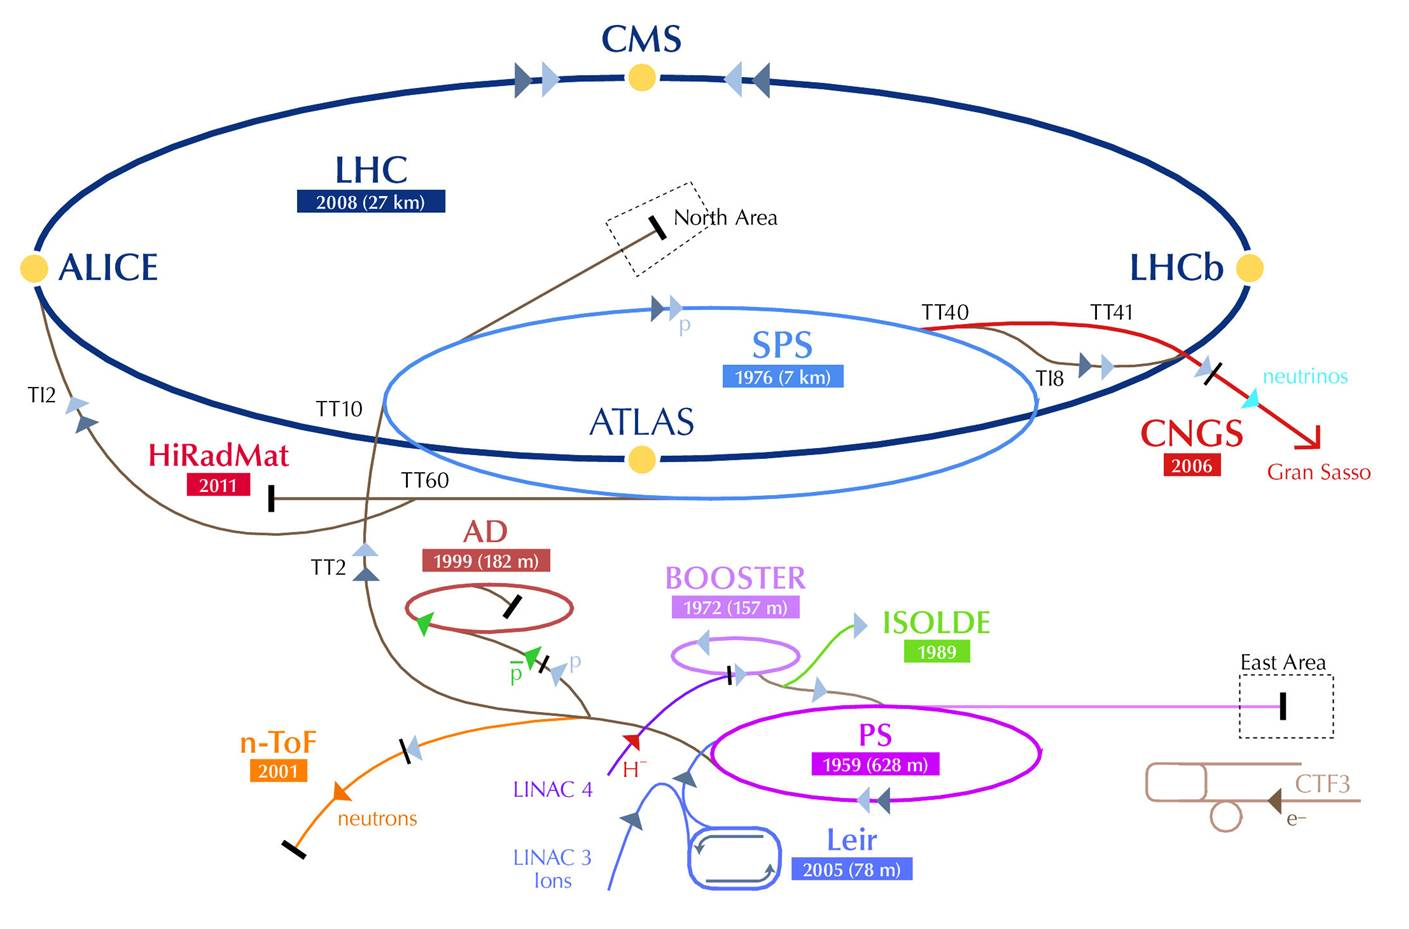
\includegraphics[width=0.7\textwidth]{/ch2/lhc_acce}
	\caption[The CERN acceleration \ital{facilities}]{The CERN acceleration \ital{facilities} showing the location of the four main experiment as well as the acceleration process[need ref].}
	\label{fig:cern}
\end{figure}

It began operation in 2010 after two years solving issues that cause a false start in 2008. The LHC prove soon to be a success and in just two years of operations dele  



The protons starts from a botle of hydrogen 

%With 27 km of circumference, the LHC is currently the most powerful circular acceler- ator in the world. It is installed in the same tunnel where the Large Electron-Positron (LEP) collider was located, taking advantage of the existing infrastructure. The LHC is part of the CERN’s accelerator complex composed of several successive accelerat- ing stages before the particles are injected into the LHC ring where they reach their maximum energy (see Figure 3.1).

Four experiments were designed and built around the LHC 27 km long acceleration ring to test different physics theories and search for undiscovered particles at the LHC. Two of them, A Toroidal Large Aparatus (ATLAS)\cite{atlas} and the Compact Muon Solenoid (CMS)\cite{cms_doc} are large multipurpose experiments. The third experiment is LHCb \cite{lhcb}, which is specifically dedicated to study B-meson physics, the last experiment ALICE \cite{alice}, A Large Ion Collider Experiment, was design to investigate heavy ion collisions.


\begin{figure}[!h]
	\centering
	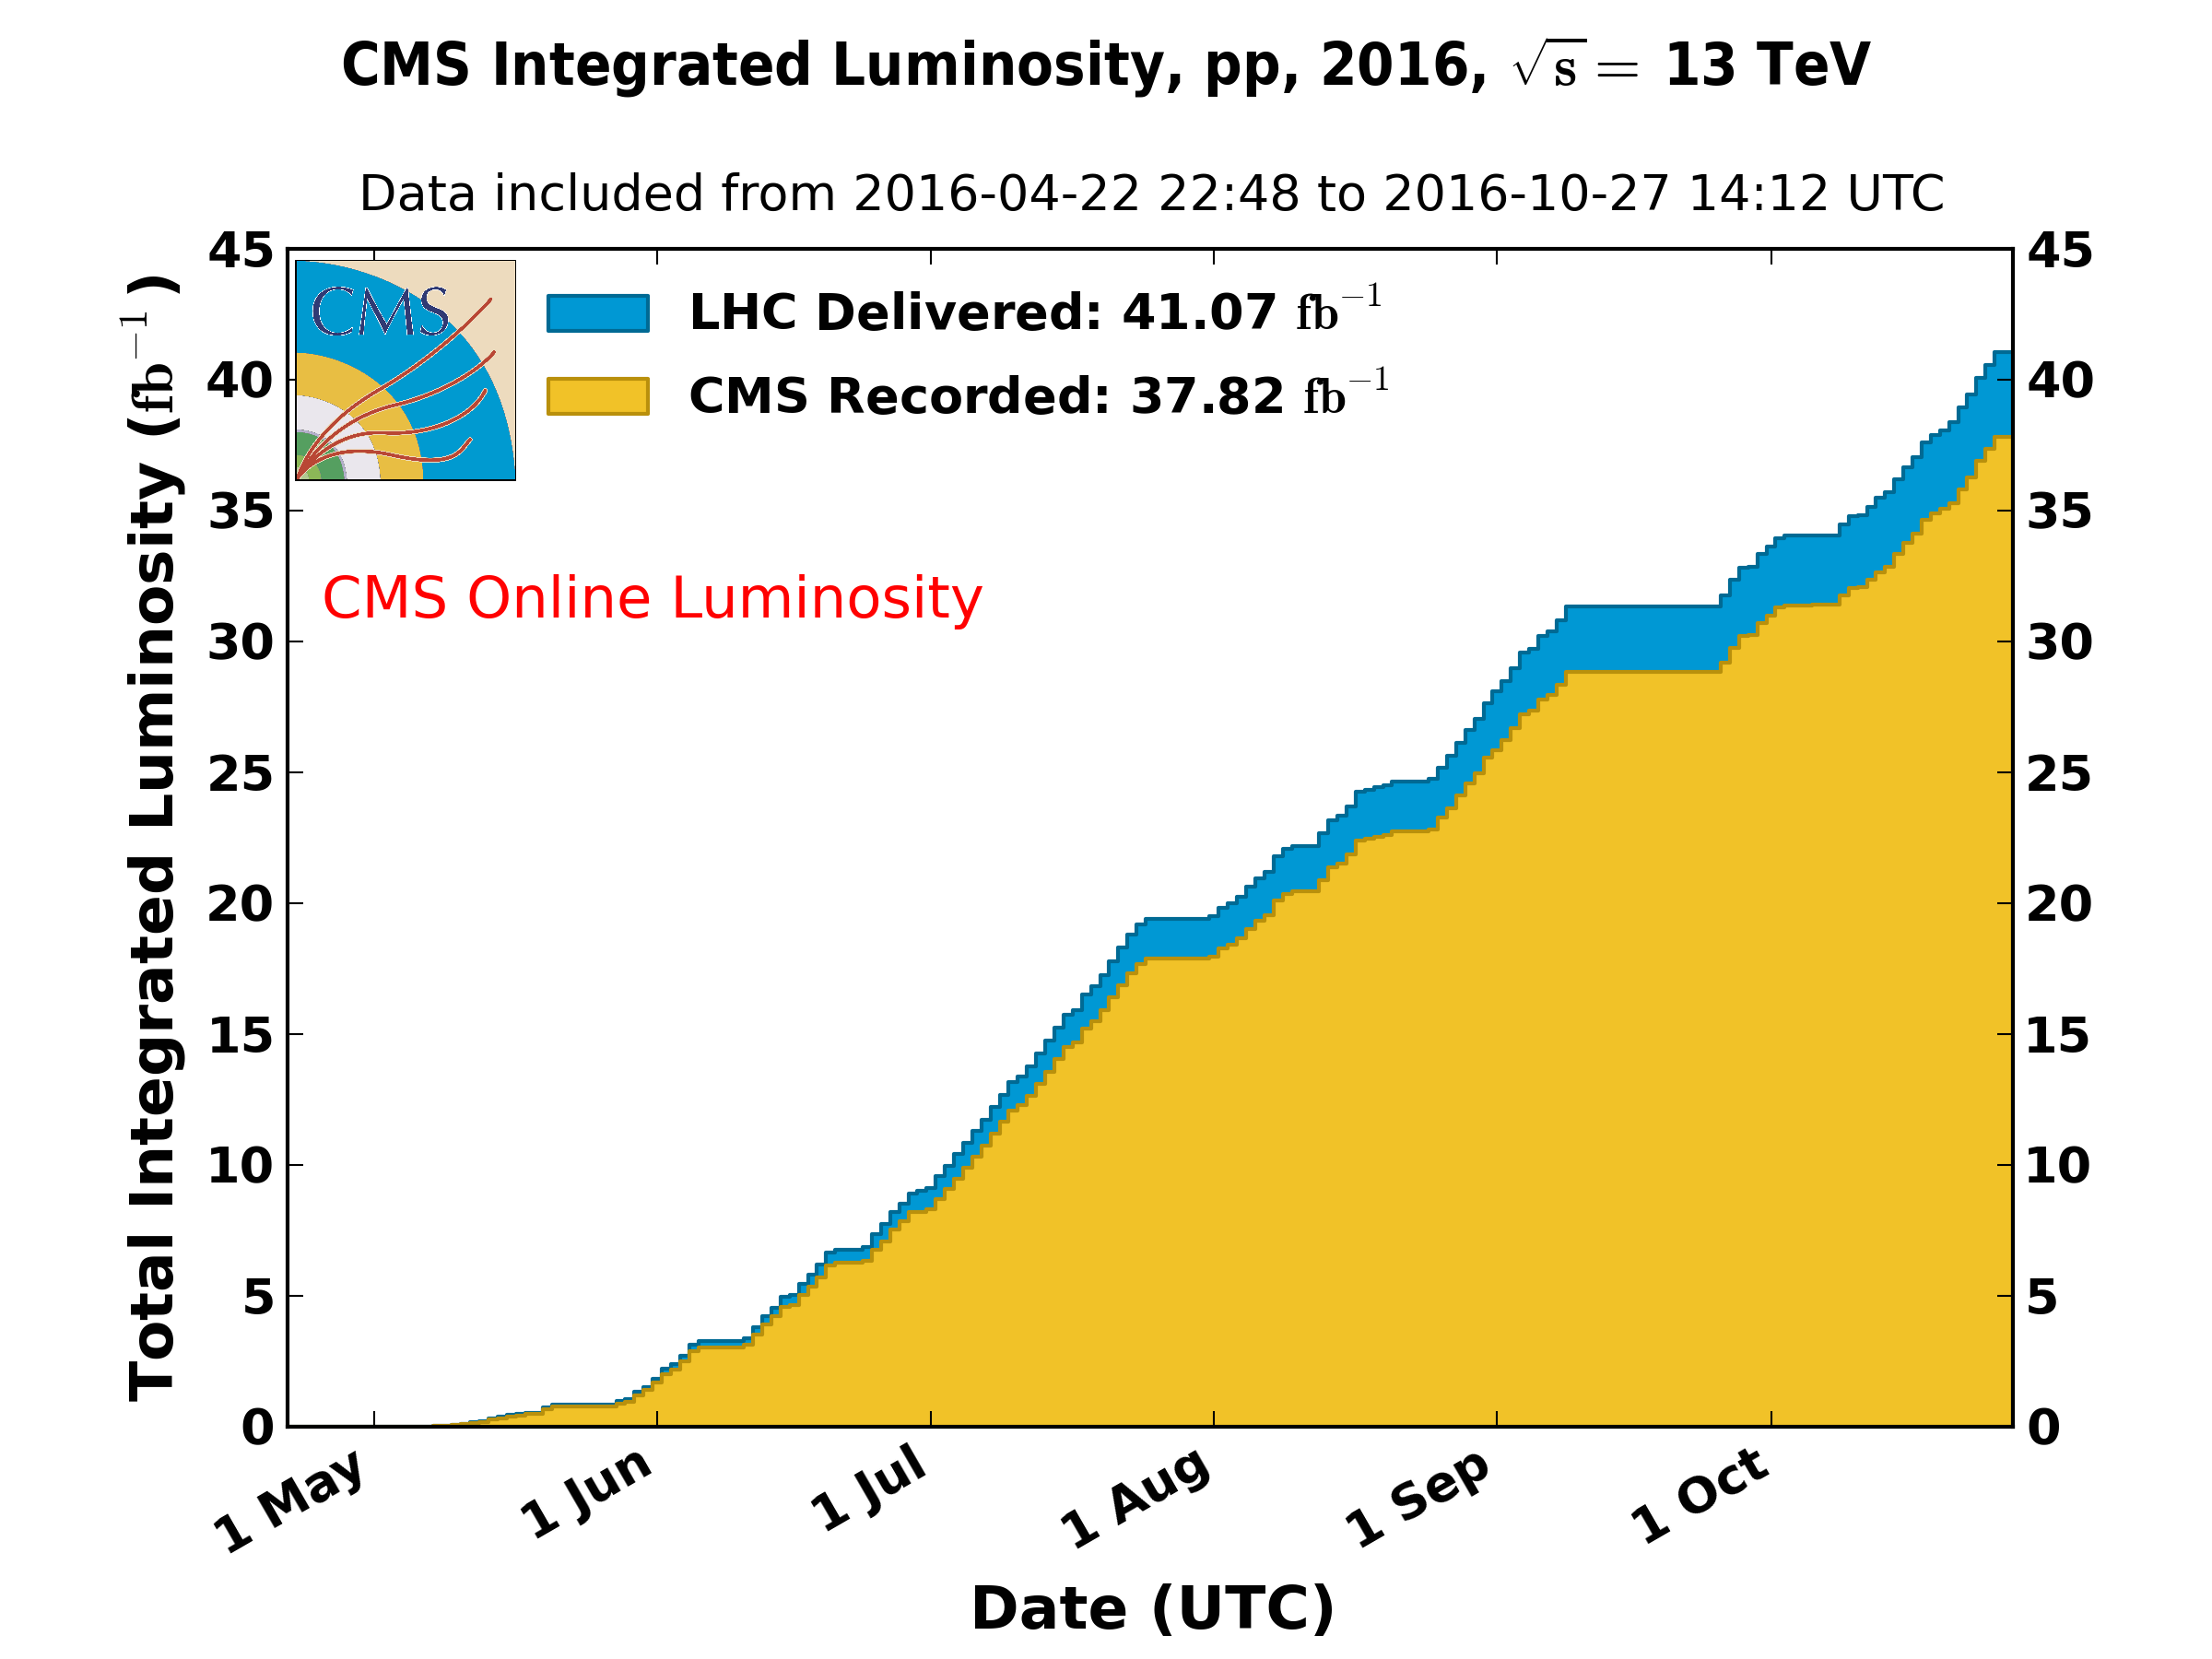
\includegraphics[width=0.7\textwidth]{ch2/lumi_2016}
	\caption[LHC luminosity]{Total integrated luminosity delivered by the LHC machine to the CMS experiment as of 2016.{\rojo{find current one}}}
	\label{lumi2016}
\end{figure}


\begin{figure}[!h]
	\centering
	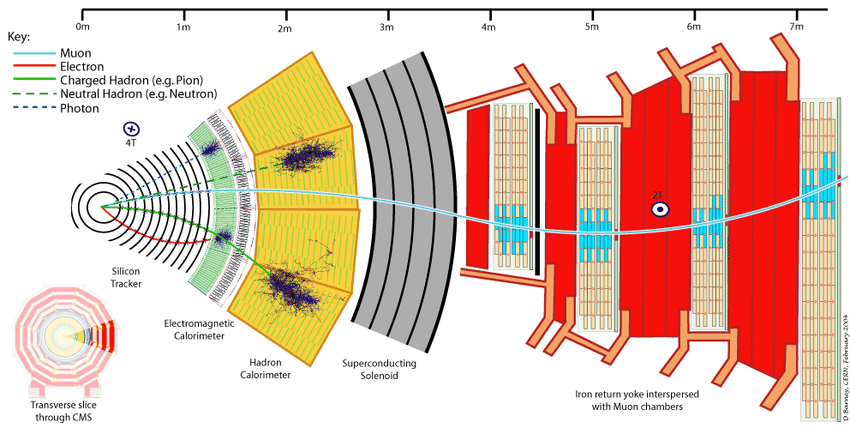
\includegraphics[width=0.7\textwidth]{ch2/cms_cross}
	\caption[LHC dipoles]{LHC dipoles.}
	\label{fig:cmscross}
\end{figure}


%\subsection{LHCb}
%\subsection{Atlas}
%\subsection{ALICE}
\section{CMS}
The compact muon soleinod is one of the two multipurpose experiment at the LHC.

images: 
run276282->An event where two Z candidates are produced and each decay into two muons, each given by the red lines. This event has 27 reconstructed vertices. (CMS SketchUp model by Tai Sakuma) (Image: CERN)
fig1 gammagamma 



\begin{figure}[!h]
	\centering
	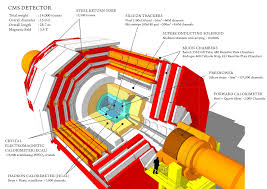
\includegraphics[width=0.7\textwidth]{ch2/cms_det}
	\caption[CMS detector]{CMS detector.}
	\label{cms_det}
\end{figure}

\begin{figure}[!h]
	\centering
	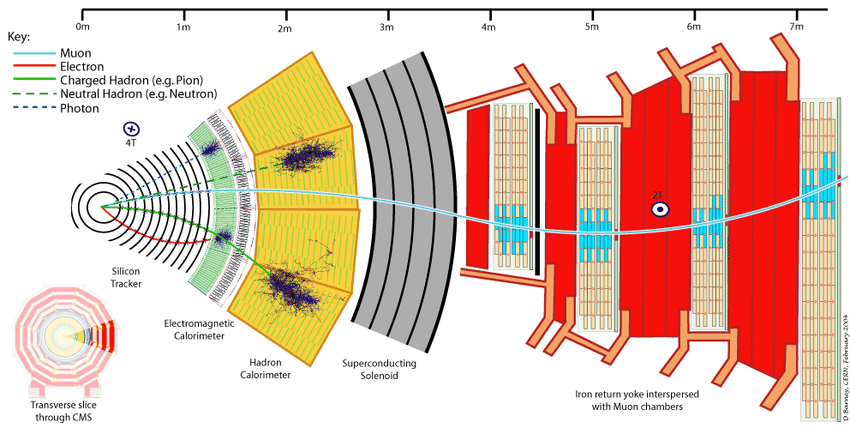
\includegraphics[width=0.7\textwidth]{ch2/cms_cross}
	\caption[CMS cross sectional view]{CMS cross sectional view.}
	\label{cmscross}
\end{figure}

\begin{figure}[h!]
	\centering
	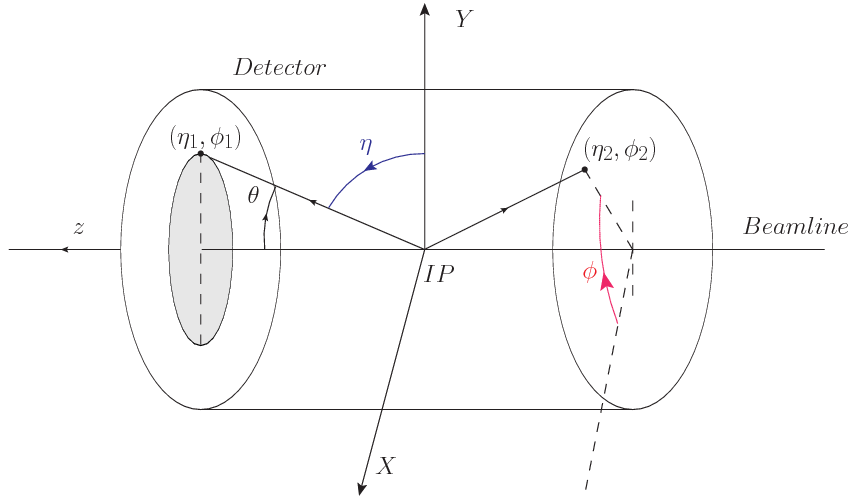
\includegraphics[scale=0.4]{ch2/coord}
	\caption[CMS detector coordinate system]{CMS detector coordinate system \cite{and_the}.}
	\label{fig:coord}
\end{figure}

Describe from the outside the CMS experiment subdetector are: the muon chambers, the hadronic calorimeter, the Electromagnetic calorimeter, the superconducting solenoid, and the tracker detector which is composed of the silicon strips and the pixel detector.

\subsection{The Muon Chambers}

%\begin{figure}[!h]
%	\centering
  %
\includegraphics[width=0.7\textwidth]{../images/ch2/9}
  %\caption[The Muon Chambers]{The Muon Chambers.}\label{fig:cms_layout}
%\end{figure}
\subsection{The Hadronic Calorimeter}
%\begin{figure}[!h]
 % \centering
  %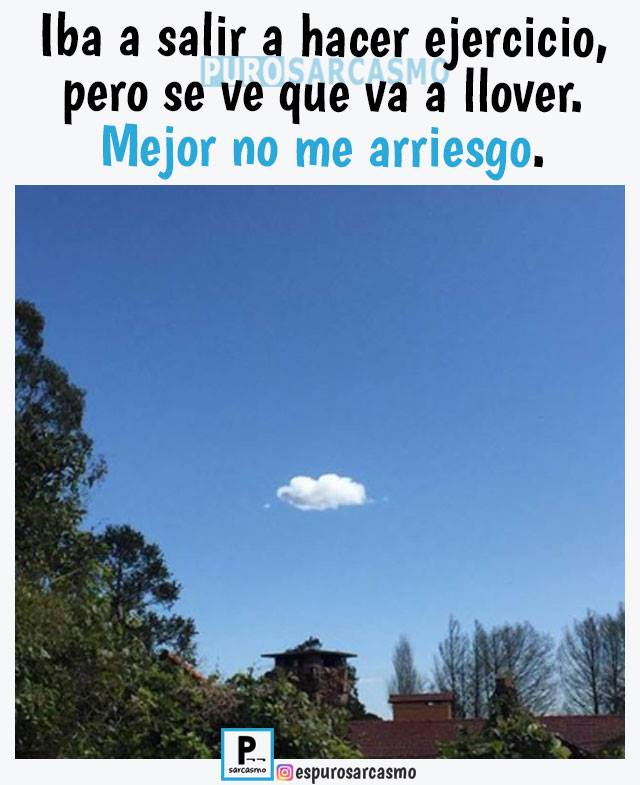
\includegraphics[width=0.7\textwidth]{../images/ch2/8}
%  \caption[The Hadronic Calorimeter]{The Hadronic Calorimeter.}\label{fig:cms_layout}
%\end{figure}

%\begin{figure}[!h]
%	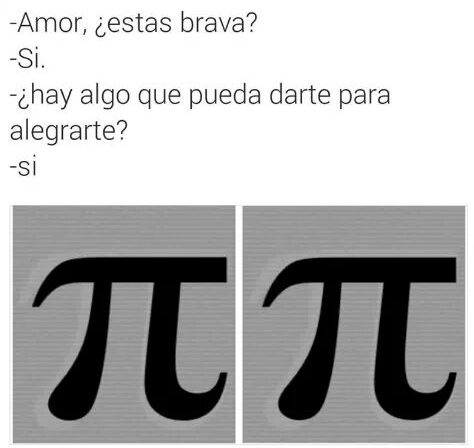
\includegraphics[width=0.7\textwidth]{ch2/8}
%  \caption[The Hadronic Calorimeter]{The Hadronic Calorimeter.}\label{fig:cms_layout}
%\end{figure}
\subsection{The Electromagnetic Calorimeter}
%\begin{figure}[!h]
%	
\includegraphics[width=0.7\textwidth]{ch2/7}
%	\caption[The Electromagnetic Calorimeter]{ The Electromagnetic Calorimeter.}\label{fig:cms_layout}
%\end{figure}

\subsection{The Tracker Detector}

%\begin{figure}[!h]
 % \centering
  %
\includegraphics[width=0.7\textwidth]{ch2/3}
  %\caption[CMS Tracking system.]{CMS Tracking system.}\label{fig:cms_layout}
%\end{figure}

\subsubsection{Silicon Strips}

%\begin{figure}[!h]
 % \centering
  %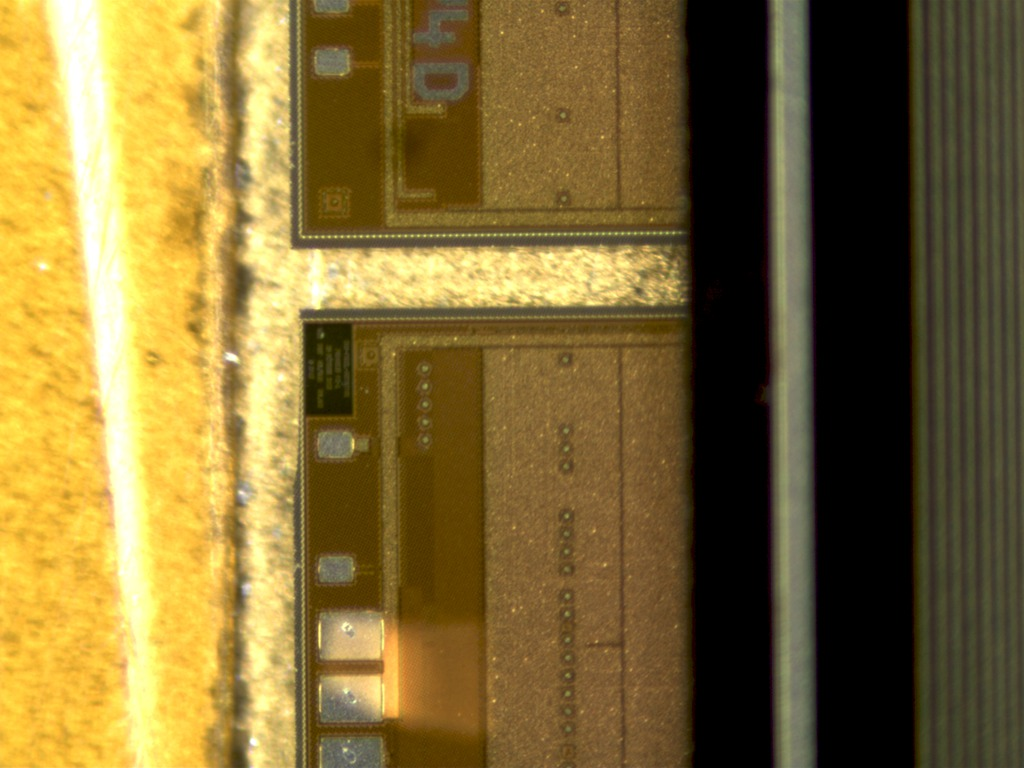
\includegraphics[width=0.7\textwidth]{ch2/6}
 % \caption[silicon strips detector]{silicon strips detecto.}\label{fig:cms_layout}
%\end{figure}

\subsubsection{Pixel Detector}
Being the innermost detector in CMS, the pixel detector works in a high radiation environment but, due to its excellent design and construction, it performed well during the initial CMS run. It provided two or more hits per track, allowing secondary vertex identification of long-lived objects. The pixel detector is composed of two parts, the barrel (BPix) and a disk at each end, denominated Forward pixel detector (FPix), as showing in figure \ref{pixeldetector}. The BPix is made of three layers located at 4.3 cm, 7.2 cm, and 11.0 cm from the interaction point respectively. The FPix has two layers, one at 34.5 cm and the other at 46.5 from the interaction point. This thesis will focus on the FPix, the part of the detector where UNL has made major contributions in the last {\rojo{two}} three decades.  

\begin{figure}[!h]
	\centering
	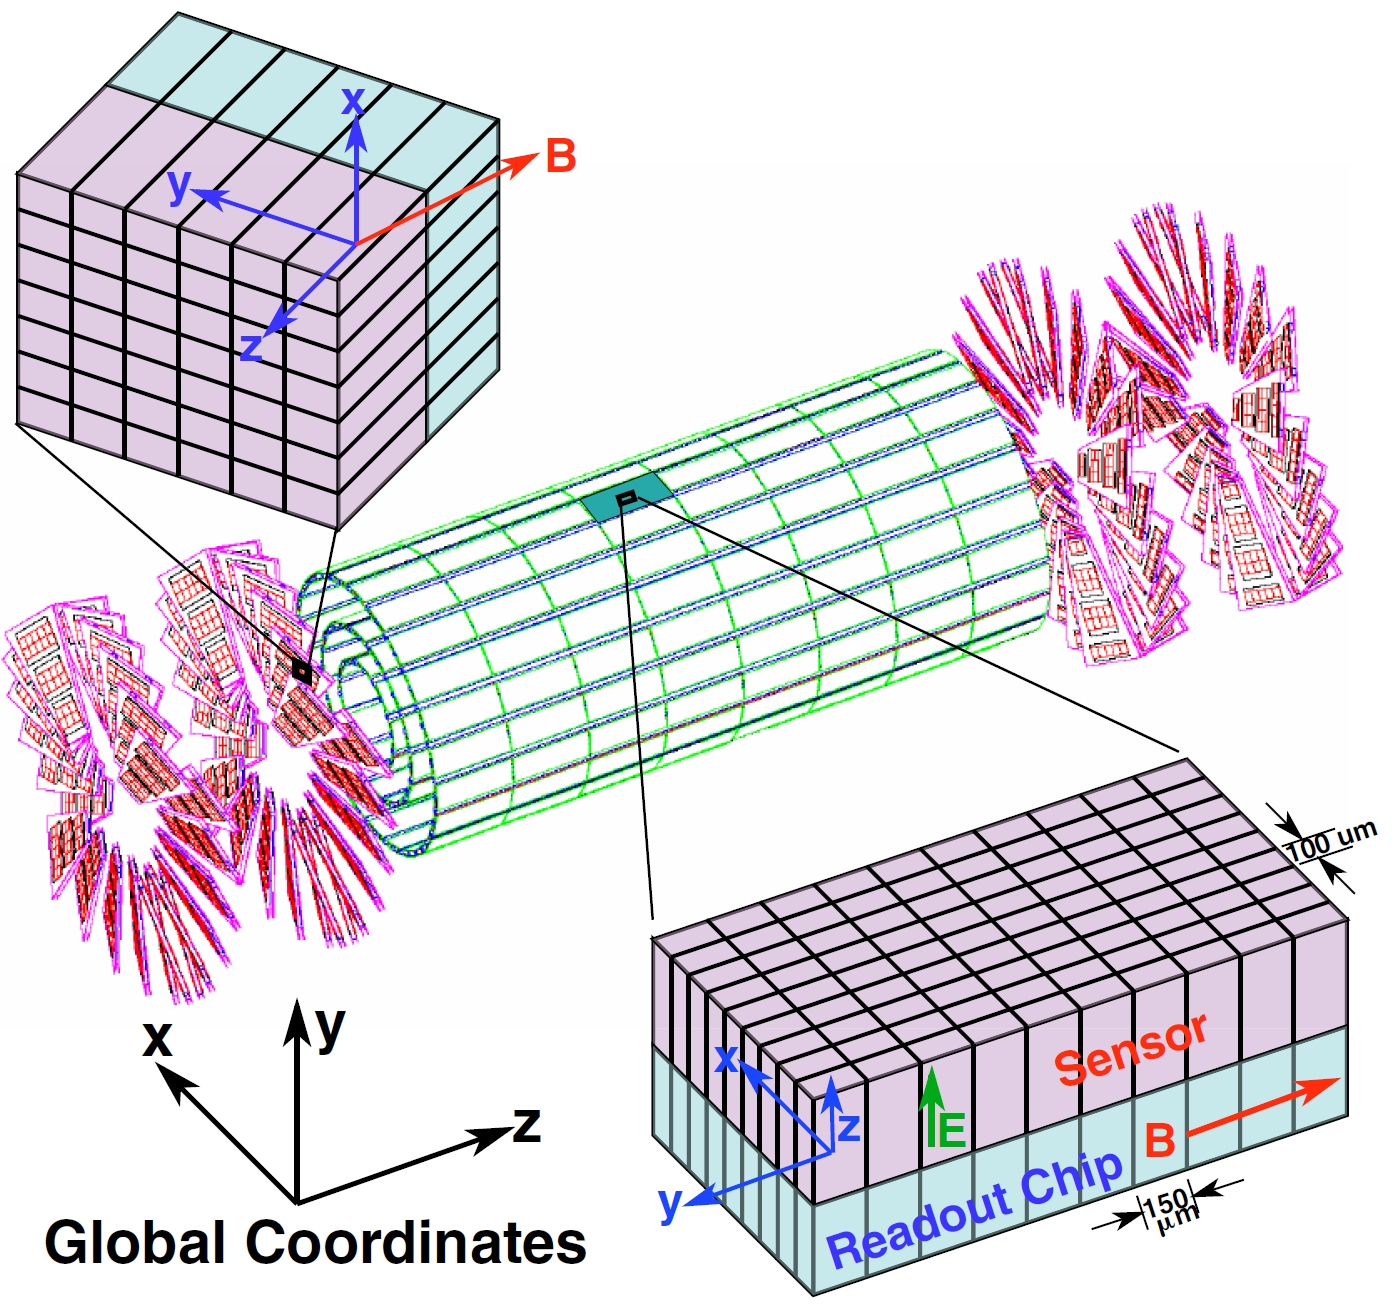
\includegraphics[width=0.7\textwidth]{ch2/pixel_detector}
	\caption[Pixel detector]{Pixel detector.}
	\label{pixeldetector}
\end{figure}

  

The original FPix, also known as phase 0, was populated by 672 modules of 100 by 100 $\mu m$ 





